% !TEX root = mythesis.tex

%==============================================================================
\chapter{Theoretical Overview}
\label{sec:theory}
%==============================================================================
\newcommand{\todo}[1]{\textbf{\color{red}TODO: #1}}

\section{Excitons}
% Terminology
An exciton is a bound state of electron and hole. This neutral quasi-particle is bosoniclike, meaning that it can occupy the same excitonic ground state. These composite particles are theorized to be formed when the binding energy of the electron-hole pair is bigger than the band gap. This results in an unstable ground state against spontaneous exciton generation (Fig. \ref{fig:exciton_gap}). It is worth noting that the ground state instability is important because the so called excitonic insulator is a candidate for observing a Bose-Einstein condensation transition~\cite{grossnev}. The excitons remind of the Cooper pairs (bound state of spin-up and spin-down electrons) used in describing superconductivity. Similarly, they form below a critical temperature and impose a quasi-particle gap~\cite{ctubes}. Unlike the Cooper pairs, they do not transport charge or mass but only energy~\cite{grossnev}. 
% put a Graphic here
\begin{figure}[htbp]
    \centerline{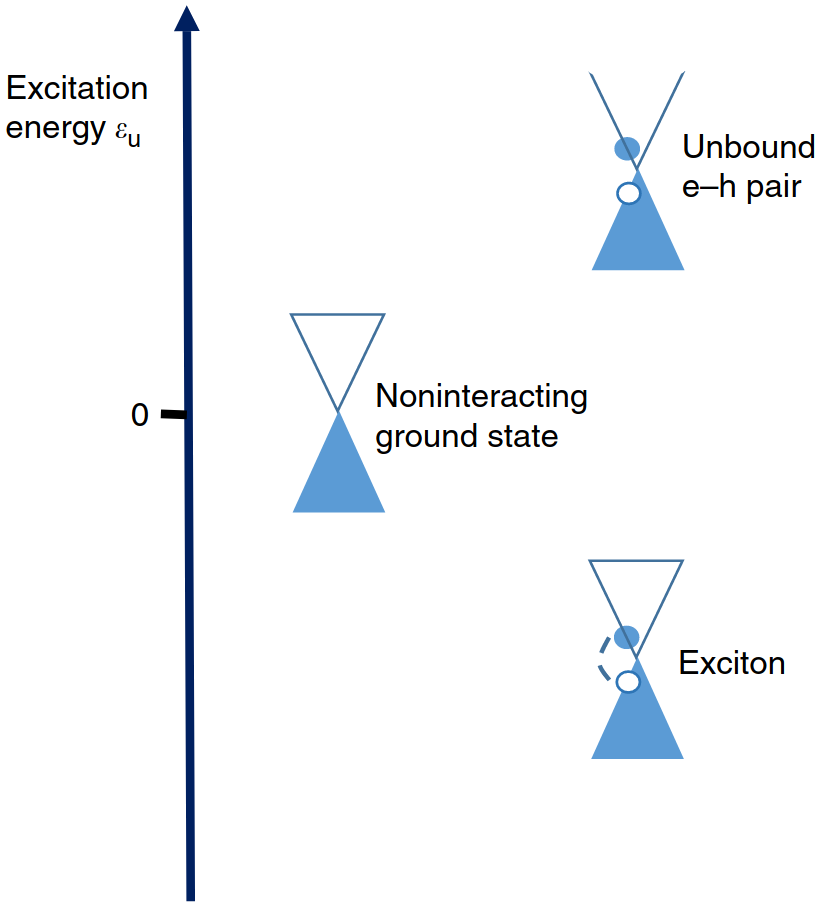
\includegraphics[width=0.35\linewidth]{exciton_gap.png}}
    % \centerline{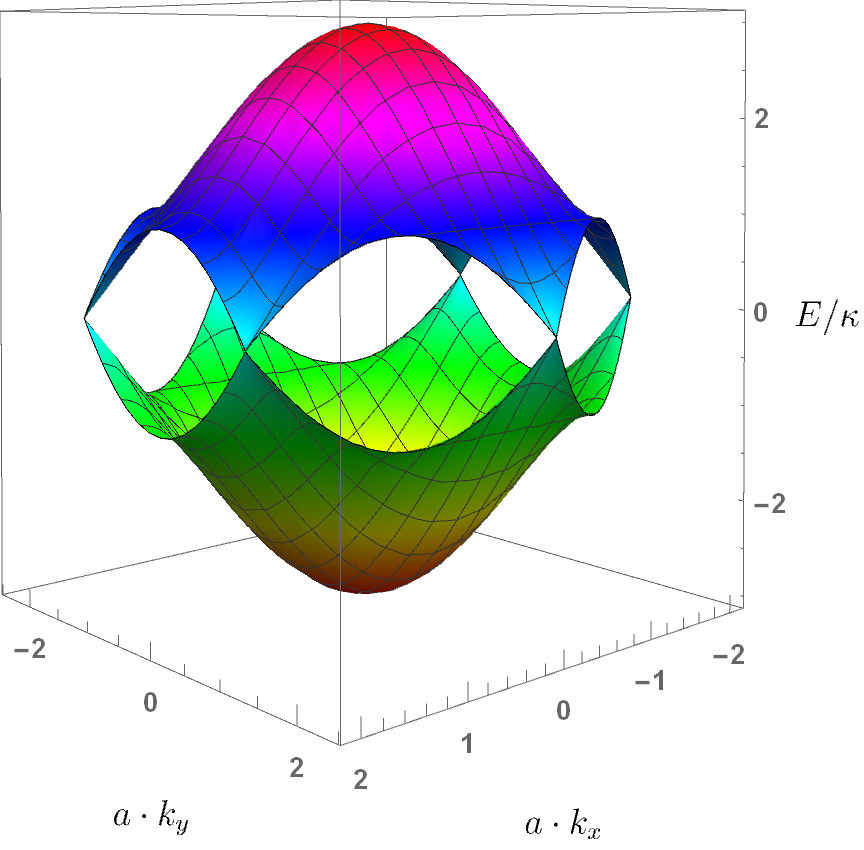
\includegraphics[width=0.7\linewidth]{band_structure.png}}
    \caption{Excitonic instability in carbon nanotubes. The scheme represents the excitation energy $\epsilon_u$ of an electron-hole (e-h) pair relative to the noninteracting ground state, a zero-gap semiconductor. In the absence of interaction, the excitation energy $\epsilon_u$ of an e-h pair is positive. The long-range interaction may bind e-h pairs close to the Dirac point in the momentum space. If an exciton forms, then its excitation energy $\epsilon_u$ is negative. This instability leads to the reconstruction of the ground state into an excitonic insulator~\cite{ctubes}. (took the caption word-for-word)}
    \label{fig:exciton_gap}
\end{figure}

% Developments
In recent years, there has been a renewed interest in investigating excitons due to their theoretically proposed applications in technology. These excitonic bound states are considered to be good candidates for the development of topologically protected qubits, switching devices, and in heat exchangers~\cite{graphapl1, graphapl2, graphapl3}. The properties of the exciton have been studied on a microscopic level by employing Hubbard-like Hamiltonians on graphene lattices~\cite{graphene1, graphene2} as well as the 3D thin-films topological insulators~\cite{graphene3, graphene4, graphene5}. There are other models (e.g. Gross-Neveu models) that have been used to describe excitons in semimetals and in semiconductors by studying the phase transitions between them and excitonic insulator. It has been shown that the dynamics of the bound electron-hole pair can be controlled in van der Waals heterostructures via a change of twist angle between the monolayers. These properties (most importantly the lifetimes of the excitons) can be tuned from the appearance of moiré potential, which in momentum space translates to relative rotation of both layer's Brillouin zones~\cite{twistangle}.
% Simulations
% On the lattice?
% Different models for excitons

In this work, we apply the Hubbard model onto a hexagonal lattice which is a model of graphene (see Section \ref{sec:lattice}). We are looking for the appearance of an electron-hole bound state. This will be done by measuring the binding energy of the correlation functions ratio
\begin{equation}
    \epsilon = (E_e + E_h) - E_{e-h} = \ln\left( \frac{C_e(\tau)C_h(\tau)}{C_{e-h}(\tau)} \right)
\end{equation}
The Hubbard model that we are applying there is not a mechanism for decay of the exciton state. This means that if the energy is negative ($\epsilon < 0$), we have a bound exciton state; and if the energy is higher than the energy threshold, then the particles are unbound. The study of a monolayer graphene sheets that we do in this thesis is a first step in the direction of future investigation of more complex graphene (and other) structures.

\section{The Hubbard Model}

% Maybe history
The Hubbard model (HM) emerges as a simple solution to the many-body problem in solids. It is a theory that describes the interactions of fermions on lattices, where they can hop between neighboring sites. This model successfully describes the ferromagnetic properties of materials with different strength correlations between electrons. % look-up if true and what to add as citation

% Original Hubbard model Hamiltonian (Tight-binding, interaction, Chemical potential)
The tight-binding with on-site interaction Hamiltonian describes the hopping of the fermions between neighboring sites and the interaction of fermions
\begin{equation}
    H = - \sum_{xy} \left( a^\dagger_{x,\uparrow} K_{xy} a_{y,\uparrow} + a^\dagger_{x,\downarrow} K_{xy} a_{y,\downarrow} \right) - \frac{1}{2} \sum_{x,y} \left( (n^\dagger_{x,\uparrow} - n^\dagger_{x,\downarrow}) V_{xy} (n^\dagger_{y,\uparrow} - n^\dagger_{y,\downarrow}) \right)
\end{equation}
where the first term is the kinetic and the second is the interaction; $a^\dagger$, $a$ are the creation and annihilation operators respectively of electrons, $\uparrow$ is indicating spin-up and $\downarrow$ is spin-down, $K$ is called the hopping matrix which describes the hopping between sites, the interaction term is represented by the potential $V$, and $n_{x,s} = a^\dagger_{x,s} a_{x,s}$ is the electron number density operator. We can make a change of basis, such that particles are separated by spin and charge, which we call a particle-hole symmetry (see Section \ref{ssec:ph-trafo})
\begin{equation}
    \begin{aligned}
        p^\dagger_x & \equiv a^\dagger_{x,\uparrow} \qquad\qquad h^\dagger_x & \equiv a_{x,\downarrow} \\
        p_x & \equiv a_{x,\uparrow} \qquad\qquad h_x & \equiv a^\dagger_{x,\downarrow}
    \end{aligned}
    \label{eq:ph-switch}
\end{equation}
where $p^\dagger (p)$, $h^\dagger (h)$ are the creation(annihilation) operators of particles and holes. Since these operators describe fermions, they respect the anti-commutation relations i.e. the Pauli exclusion principle

\begin{equation}
    \begin{aligned}
        \{ p^\dagger_x, p_y \} &= \delta_{xy} &\{ h^\dagger_x, h_y \} = \delta_{xy}
        \\
        \{ p_x, p_y \} &= \{ p^\dagger_x, p^\dagger_y \} = 0 &\{ h_x, h_y \} = \{ h^\dagger_x, h^\dagger_y \} = 0
        \\
        \{ p^\dagger_x, p_y \} &= \{ p^\dagger_x, h^\dagger_y \} = 0 \qquad\qquad &\{ p_x, h_y \} = \{ p_x, h^\dagger_y \} = 0
        \\
    \end{aligned}
\end{equation}
% Particle-hole basis (Creation and annihilation operators)
The convention for spin and charge that we use for the particles and holes operators is given in Table \ref{tab:convention_operators}.
\begin{table}[h]
    \centering
    \begin{tabular}{c|ccc}
        & $Q$ & $S$ & $S^3$ \\
    \hline
        $p^\dagger$ & +1 & $\frac{1}{2}$ & $-\frac{1}{2}$ \\
        $p$ & -1 & $\frac{1}{2}$ & $+\frac{1}{2}$ \\
        $h^\dagger$ & -1 & $\frac{1}{2}$ & $-\frac{1}{2}$ \\
        $h$ & +1 & $\frac{1}{2}$ & $+\frac{1}{2}$ \\
    \end{tabular}
    \caption{Convention of charge ($Q$), spin ($S$), and third component of spin ($S^3$) used for creation and annihilation operators of particles and holes.}
    \label{tab:convention_operators}
\end{table}
Here $Q$, $S$, $S^3$ are the charge, spin, and the third component of the spin respectively. For the two-body correlators (discussed in Section \ref{sec:corr_func}), it is also convenient to know the quantum numbers for different combinations of particle and hole operators. In Table \ref{tab:ph-comb} is given a summary which will be useful in the next chapters. We notice that only the charge and $S^3$ are present in the table. This is due to $Q$ and $S^3$ being additive numbers, whereas the spin is not because two different spin values could have the same third component (ex. $S=0,1;S^3=0$).
\begin{table}[h]
    \centering
    \begin{tabular}{c|cc}
        & $Q$ & $S^3$ \\
    \hline
        $p^\dagger p^\dagger$ & +2 & $-1$ \\
        $p^\dagger p$ & 0 & $0$ \\
        $p^\dagger h^\dagger$ & 0 & $-1$ \\
        $p^\dagger h$ & +2 & $0$ \\
        $p p$ & -2 & $+1$ \\
        $p h^\dagger$ & -2 & $0$ \\
        $p h$ & 0 & $+1$ \\
        $h^\dagger h^\dagger$ & -2 & $-1$ \\
        $h^\dagger h$ & 0 & $0$ \\
        $h h$ & +2 & $+1$ \\
    \end{tabular}
    \caption{Quantum numbers for the combination of particle and hole operators.}
    \label{tab:ph-comb}
\end{table}

% Particle-hole Hubbard Hamiltonian
We can now substitute the operators inside the Hamiltonian with the ones in the new basis
\begin{equation}
    H = - \sum_{xy} \left( p^\dagger_x K_{xy} p_y - h^\dagger_x K_{xy} h_y \right) + \frac{1}{2} \sum_{x,y} \left( (n^\dagger_{x,p} - n^\dagger_{x,h}) V_{xy} (n^\dagger_{y,p} - n^\dagger_{y,h}) \right),
\end{equation}
here we have added a new index to the number density operators which indicates whether particles or holes are counted.

Finally, we can expand our Hamiltonian with one more term, which is called the chemical potential term, where $\mu$ is the chemical potential. It accounts for the change of the number of particles and holes
\begin{equation}
    H - \vec{\mu}\cdot\vec{q} = - \sum_{xy} \left( p^\dagger_x K_{xy} p_y + h^\dagger_x K_{xy} h_y \right) + \frac{1}{2}\sum_{xy} q_x V_{xy} q_y - \sum_{x} \mu_x q_x
\end{equation}
and we have introduced one more operator $q_x = n_{x,p} - n_{x,h}$. This is the charge operator that indicates the relative charge on each site. 

The Hamiltonian of this model for our ease can be divided into two parts -- the half-filling part of the whole Hamiltonian and the chemical potential part. The former contains the kinetic and the interaction terms, whereas the latter in made out of only the chemical term. In the case of bipartite lattices (Chapter "SYMMETRY"), we must be able to differentiate on which lattice sites the operators are. This could be done by modifying the transformation (\ref{eq:ph-switch}) to include site dependent sign $\sigma_k$ for holes
\begin{equation}
    H - \vec{\mu}\cdot\vec{q} = - \sum_{xy} \left( p^\dagger_x K_{xy} p_y + \sigma_k h^\dagger_x K_{xy} h_y \right) + \frac{1}{2}\sum_{xy} q_x V_{xy} q_y - \sum_{x} \mu_x q_x.
\end{equation}

To get to the Hamiltonian that we work with, we choose to have only contact interactions ($V_{xy} = U\delta_{xy}$). This means that the interactions are done only in the same site
\begin{equation}
    H - \vec{\mu}\cdot\vec{q} = - \sum_{xy} \left( p^\dagger_x K_{xy} p_y + \sigma_k h^\dagger_x K_{xy} h_y \right) + \frac{U}{2}\sum_{xy} q^2_x - \sum_{x} \mu_x q_x.
\end{equation}
In this thesis work we sometimes work with the chemical potential, and sometimes we set $\mu = 0$, depending on the symmetries that we use \cite{avoiding ergodicity}. On Figure \ref{fig:hub_scheme} is shown a schematic of the Hubbard model's hopping and interaction.
\begin{figure}[h]
    \begin{center}
        \begin{tikzpicture}
            \tikzstyle{arrow} = [very thick,->,>=stealth]
            \def \spacing{2}
            \draw[step=\spacing,gray,very thin,dashed] (-0.5,-0.5) grid (6.5,6.5);

            \fill[color=black] (0*\spacing,1*\spacing) circle (0.15);
            \draw[color=black] (1*\spacing,1*\spacing) circle (0.15);
            \fill[color=white] (1*\spacing,1*\spacing) circle (0.15);
            \fill[color=black] (2*\spacing,2*\spacing) circle (0.15);
            \draw[color=black] (2*\spacing,3*\spacing) circle (0.15);
            \fill[color=white] (2*\spacing,3*\spacing) circle (0.15);
            \fill[color=black] (1.05*\spacing,2.05*\spacing) circle (0.15) node[anchor=south east] {\textbf{$V$}};
            \draw[color=black] (0.95*\spacing,1.95*\spacing) circle (0.15);
            \fill[color=white] (0.95*\spacing,1.95*\spacing) circle (0.15);
            \draw[color=black] (3*\spacing,1*\spacing) circle (0.15);
            \fill[color=white] (3*\spacing,1*\spacing) circle (0.15);
            \fill[color=black] (0*\spacing,3*\spacing) circle (0.15);
            \draw[color=black] (1.95*\spacing,-0.05*\spacing) circle (0.15);
            \fill[color=white] (1.95*\spacing,-0.05*\spacing) circle (0.15);
            \fill[color=black] (2.05*\spacing,0.05*\spacing) circle (0.15) node[anchor=south east] {\textbf{$V$}};
 
            \draw[arrow, shorten >=5pt, shorten <=5pt] (0*\spacing,1*\spacing) to [bend left=30] node [midway, sloped, above] {$K$} (1*\spacing,1*\spacing);
            \draw[arrow, shorten >=5pt, shorten <=5pt] (2*\spacing,3*\spacing) to [bend left=30] node [midway, right] {$K$} (2*\spacing,2*\spacing);
        \end{tikzpicture}
        \caption{Schematic view of the hopping and the interaction of electrons with different spin on a square lattice. Here $K$ is the hopping matrix containing the hopping probabilities and $V$ is the interaction potential. In the particle-hole basis the black and white dots represent particles and holes.}
        \label{fig:hub_scheme}
    \end{center}
\end{figure}
% Problems
The theory that we are working with as mentioned before is a model of the real physical systems. Even though the HM gives us good results, one must know some drawbacks of the model. One is that it neglects the long range part of the Coulomb forces. It is likely that significant effects are missed by this simplification [MOTT]. Another weakness of this model it has difficulties being applied to transition metals. And the Hubbard model cannot be exactly solved, so approximations must be used.

Despite having these issues, the two-dimensional HM has showed promising results when applied to honeycomb lattices. The description of the electronic structure when applied resembles that of the carbon nano structures, such as graphene, carbon nano tubes, and ribbons.
% Examples of Hubbard model
% Solutions to the model (Exact, not so exact)

% The next part should be tested more
An exact solution to the Hubbard model Hamiltonian exists in the non-interacting case at half filling. Even though, the data and analysis are done with the full Hamiltonian, it is always helpful to know the behavior of the model in the non-interacting case. The pattern that emerges is usually kept in the interacting case, and this will give us something to compare to. Since we are applying HM on the hexagonal lattice (see section LATTICE) in this work, we have the following two-band dispersion relation
\begin{equation}
    E_{\vec{k}\pm} = \pm (-\kappa) \sqrt{3 + 2 \left( \cos\left( \frac{3}{2}k_x + \frac{\sqrt{3}}{2}k_y \right) + \cos\left( \frac{3}{2}k_x - \frac{\sqrt{3}}{2}k_y \right) + \cos\left( \sqrt{3}k_y \right) \right)},
\end{equation}
where $k$ is the momentum mode and $\kappa$ is the hopping parameter. In Figure \ref{fig:two-band}, it is shown how the exact solution of the band structure looks like for infinite and finite volume lattices. One notices that for infinite lattice volume the momentum modes are continuously filled, and the model gets the full symmetry of the lattice. Whereas in the finite volume regime only a finite number of momentum modes are available to us. The symmetry is also kept in the finite volume regime with lattices that have $L_1 = L_2$; and for every other configuration of hexagonal lattice, the full symmetry is broken to other symmetries. We expect to keep the two-band structure, even if we add the interaction term and chemical potential term. Therefore, we must add a label to the ladder operators indicating the band that they are applied to. For further information on the symmetries of the lattice and the model, see chapter SYMMETRY.
% Creation and annihilation operators convention
\begin{figure}[htbp]
    \centerline{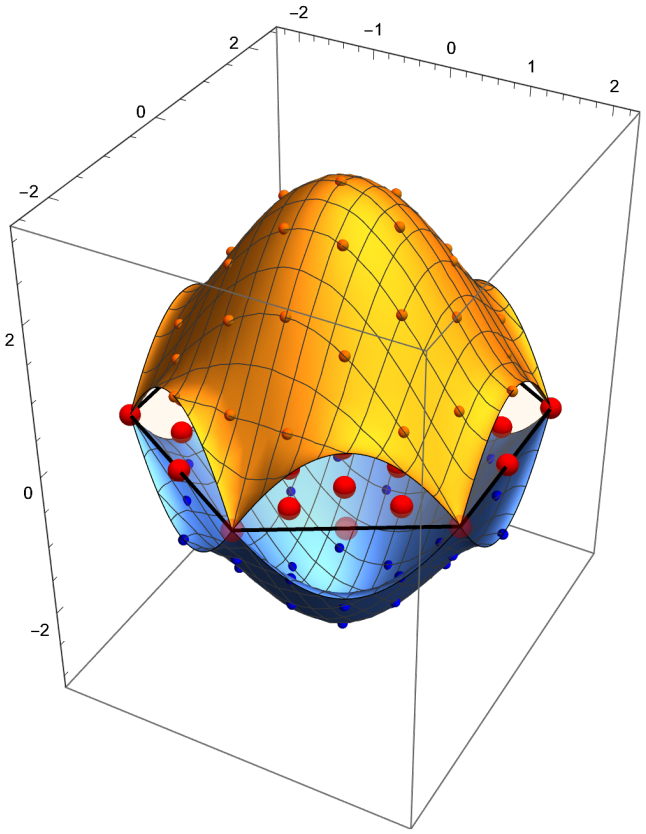
\includegraphics[width=0.5\linewidth]{two-band-structure.png}}
    % \centerline{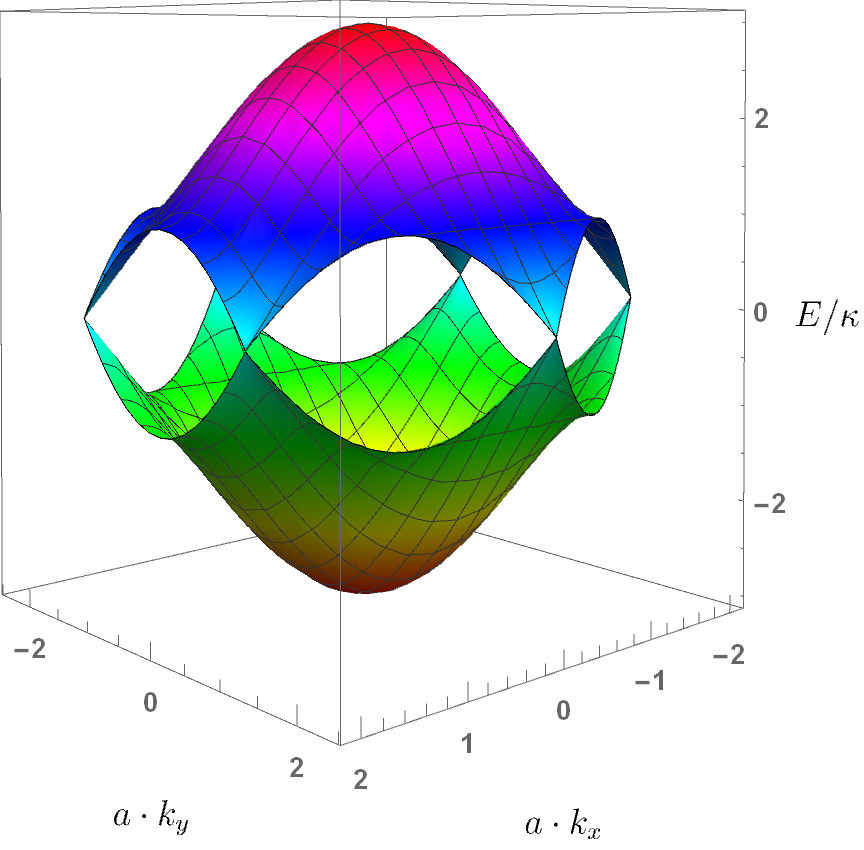
\includegraphics[width=0.7\linewidth]{band_structure.png}}
    \caption{The noninteracting one-body spectrum on the honeycomb lattice. The BZ is shown as a black hexagon, while the red spheres are the momenta allowed on a $L_1 = 6$, $L_2 = 6$ lattice and the orange and blue spheres are the corresponding non-interacting energies. [EVAN'S PAPER]}
    \label{fig:two-band}
\end{figure}


\section{Corelation Functions}
\label{sec:corr_func}

The correlation functions (correlators) that we are interested in ($\langle \mathcal{O}_{x,t+\tau}\mathcal{O}^\dagger_{y,t} \rangle$), are called Euclidean correlators. They are defined as a thermal trace
\begin{equation}
    \langle \mathcal{O}_{x,t+\tau}\mathcal{O}_{y,t} \rangle = \frac{1}{\mathcal{Z}}tr\left[ \mathcal{O}_{x,t+\tau}\mathcal{O}_{y,t}\mathrm{e}^{-\beta H} \right],
\end{equation}
where the $\mathcal{O}$ operators could be operators that create or annihilate states (usually the adjoint operator creates the anti-state), measure observables, or a combination of these; the labels $x$ and $y$ are there to indicate any set of labels, not just a position, $\mathcal{Z} = tr\left[ \mathrm{e}^{-\beta H} \right]$ is the partition function, $\beta$ is the inverse temperature, and $H$ is a general Hamiltonian of a model. In our case model, the field operators create states with a set of quantum numbers that define it at some time $t$ and destroy the same states at a different time $t + \tau$. These operators can also be composite $\mathcal{O} = \mathcal{O'}_1\mathcal{O'}_2\hdots\mathcal{O'}_n$. We can make a time transformation (assuming the action is time-translation invariant), such that the source is at time zero and the sink is at time $\tau$. Then, we move to the Heisenberg picture, so the correlator becomes
\begin{equation}
    C_{xy}(\tau) := \langle \mathcal{O}_{x,\tau}\mathcal{O}_{y,0} \rangle = \frac{1}{\mathcal{Z}}tr\left[ \mathcal{O}_{x,\tau}\mathrm{e}^{-H\tau}\mathcal{O}_{y,0}\mathrm{e}^{-H(\beta - \tau)} \right]
\end{equation}
We drop the time labels that are on the operators, since we work with the Hubbard model, and we can always make the time translation that we have discussed.

In order to be able to extract energies from the correlators, we must first find the spectral decomposition. This could be done by inserting the identity operator $\mathds{1}$ written in terms of complete set of orthonormal basis
\begin{equation}
    \mathds{1} = \sum_\alpha | n \rangle \langle n |
\end{equation}
in between the operators of the expanded in the eigenbasis of the Hamiltonian thermal trace
\begin{equation}
    \begin{aligned}
        C_{xy}(\tau) &= \frac{1}{\mathcal{Z}}tr\left[ \mathcal{O}_x\mathrm{e}^{-H\tau}\mathcal{O}_y\mathrm{e}^{-H(\beta - \tau)} \right] 
        \\
        &= \frac{1}{\mathcal{Z}}\sum_\alpha\langle \alpha | \mathcal{O}_x\mathrm{e}^{-H\tau}\mathcal{O}_y\mathrm{e}^{-H(\beta - \tau)} | \alpha \rangle 
        \\
        &= \frac{1}{\mathcal{Z}}\sum_{\alpha mnl} \langle \alpha | \mathcal{O}_x | m \rangle \langle m | \mathrm{e}^{-H\tau} | n \rangle \langle n | \mathcal{O}_y | l \rangle \langle l | \mathrm{e}^{-H(\beta - \tau)} | \alpha \rangle 
        \\
        &= \frac{1}{\mathcal{Z}}\sum_{\alpha mnl}\langle \alpha | \mathcal{O}_x | m \rangle \delta_{mn}\mathrm{e}^{-E_n\tau} \langle n | \mathcal{O}_y | l \rangle \delta_{l\alpha}\mathrm{e}^{-E_\alpha(\beta - \tau)}
        \\
        &= \frac{1}{\mathcal{Z}}\sum_{\alpha n}\langle \alpha | \mathcal{O}_x | n \rangle \langle n | \mathcal{O}_y | \alpha \rangle \mathrm{e}^{-E_n\tau} \mathrm{e}^{-E_\alpha(\beta - \tau)}
        \\
        &= \frac{1}{\mathcal{Z}}\sum_{\alpha n} \mathfrak{u}_{\alpha xn} \mathfrak{u}_{ ny\alpha} \mathrm{e}^{-E_n\tau} \mathrm{e}^{-E_\alpha(\beta - \tau)},
        \\
    \end{aligned}
    \label{eq:fit_exponent}
\end{equation}
where $\mathfrak{u}_{\alpha xn}$ and $\mathfrak{u}_{ ny\alpha}$ are the overlap factors. In the limit $\beta \to \infty$, one of the exponents vanishes, meaning the lowest excited state dominates
\begin{equation}
    \lim_{\beta \to \infty} C_{xy}(\tau) = \sum_{n} \mathfrak{u}_{\Omega xn} \mathfrak{u}_{ ny\Omega} \mathrm{e}^{-\Delta E_n\tau}
    \label{eq:beta_lim}
\end{equation}
where $\Delta E_n = E_n - E_\Omega$, and $\Omega$ denotes the lowest energy state (vacuum state)~\cite{evan}.

Another way to express the two-point correlator is by using a Euclidean path integral
\begin{equation}
    C_{xy}(\tau) = \langle \mathcal{O}_x\mathcal{O}^\dagger_y \rangle = \frac{1}{\mathcal{Z}} \int \mathcal{D}\phi \:\mathrm{e}^{-S[\phi]}\times \left(\mathcal{O}_x\mathcal{O}^\dagger_y\right)_{Wick},
    \label{eq:path-int}
\end{equation}
where $\mathcal{D}\phi$ is the path integral measure, $S[\phi]$ is the Euclidean action, $\mathcal{Z}$ is the partition function defined as
\begin{equation}
    \mathcal{Z} = \int \mathcal{D}\phi \:\mathrm{e}^{-S[\phi]};
\end{equation}
the label $Wick$ indicates that all possible Wick contractions must be performed on the operators, where each term is a product of inverse fermion matrices ($M^{-1}$) \cite{gattringer}. As this is very important to the part where we generate data, we will explicitly work out two examples -- one for a one-body correlation function and the other for a two-body correlator with two Wick contractions.

\begin{itemize}
    \item \textbf{One-body correlation function}\\
    We start by substituting the general operator $\mathcal{O}$ with the particle ladder operator $p$ and their adjoints. Then, we construct the correlation function and use Wick's theorem to perform the contractions
    \begin{equation}
        \begin{aligned}
            \langle p_{x}p^\dagger_{y} \rangle &= \frac{1}{\mathcal{Z}} \int \mathcal{D}\phi \:\mathrm{e}^{-S[\phi]}\times \left(p_{x}p^\dagger_{y}\right)_{Wick} 
            \\
            &= \frac{1}{\mathcal{Z}} \int \mathcal{D}\phi \:\mathrm{e}^{-S[\phi]} M[\phi]^{-1}_{(x,y)},
        \end{aligned}
    \end{equation}
    where $x$,$y$ denote the position of the particle and $M[\phi]$ is the fermion matrix. The same derivation can be performed for $\langle h_xh^\dagger_y\rangle$.
    
    \item \textbf{Two-body correlation function}\\
    In this example, we want to show what the Wick contractions are for composite operators. We start again by substituting the general operators from \ref{eq:path-int} with $pp$ and the adjoint. Then, we expand the $\left(\dots\right)_{Wick}$, and finally we substitute $M[\phi]^{-1}$ in each term
    \begin{equation}
        \begin{aligned}
            \langle p_{1,x}p_{2,x'}p^\dagger_{3,y}p^\dagger_{4,y'} \rangle &= \frac{1}{\mathcal{Z}} \int \mathcal{D}\phi \:\mathrm{e}^{-S[\phi]}\times \left(p_{1,x}p_{2,x'}p^\dagger_{3,y}p^\dagger_{4,y'}\right)_{Wick} 
            \\
            &= \frac{1}{\mathcal{Z}} \int \mathcal{D}\phi \:\mathrm{e}^{-S[\phi]}\times \left(\wick{\c1 p_{1,x} \c2 p_{2,x'} \c2 p^\dagger_{3,y} \c1 p^\dagger_{4,y'} - \c3 p_{1,x} \c4 p_{2,x'} \c3 p^\dagger_{3,y} \c4 p^\dagger_{4,y'}}\right)_{Wick} 
            \\
            &= \frac{1}{\mathcal{Z}} \int \mathcal{D}\phi \:\mathrm{e}^{-S[\phi]} \left((M[\phi]^{-1}_{14})_{(x,y')}(M[\phi]^{-1}_{23})_{(x',y)} - (M[\phi]^{-1}_{13})_{(x,y)}(M[\phi]^{-1}_{24})_{(x',y')}\right)
        \end{aligned}
    \end{equation}
    where the number labels indicate which operators are replaced with the fermion propagator; the relative minus sign between the terms is due to the odd permutation.
\end{itemize}

The representation of the correlation functions as path integral is as mentioned important to us because we have a way to generate the correlation functions. This can be done by numerically solving the integrals using stochastic methods (see Section \ref{sec:hmc}) for Gausian integration. Then, it is possible to extract the energies of the correlators if we fit \ref{eq:fit_exponent} for different $\beta$ and volumes, and, finally, extrapolate to zero temperature (\ref{eq:beta_lim}) and infinite volume. This will give us the result we are looking for.

% One particle gap

% Fermionic matrix (Path integral, Inversion)
% Two particle gap
% Exponential representation of the correlator
% Effective mass
% Binding energy
